\chapter{Vision transformer}



\section{Transformer}

\begin{description}
    \item[Transformer] \marginnote{Transformer}
        Neural architecture designed for NLP sequence-to-sequence tasks. It heavily relies on the attention mechanism.
        \begin{figure}[H]
            \centering
            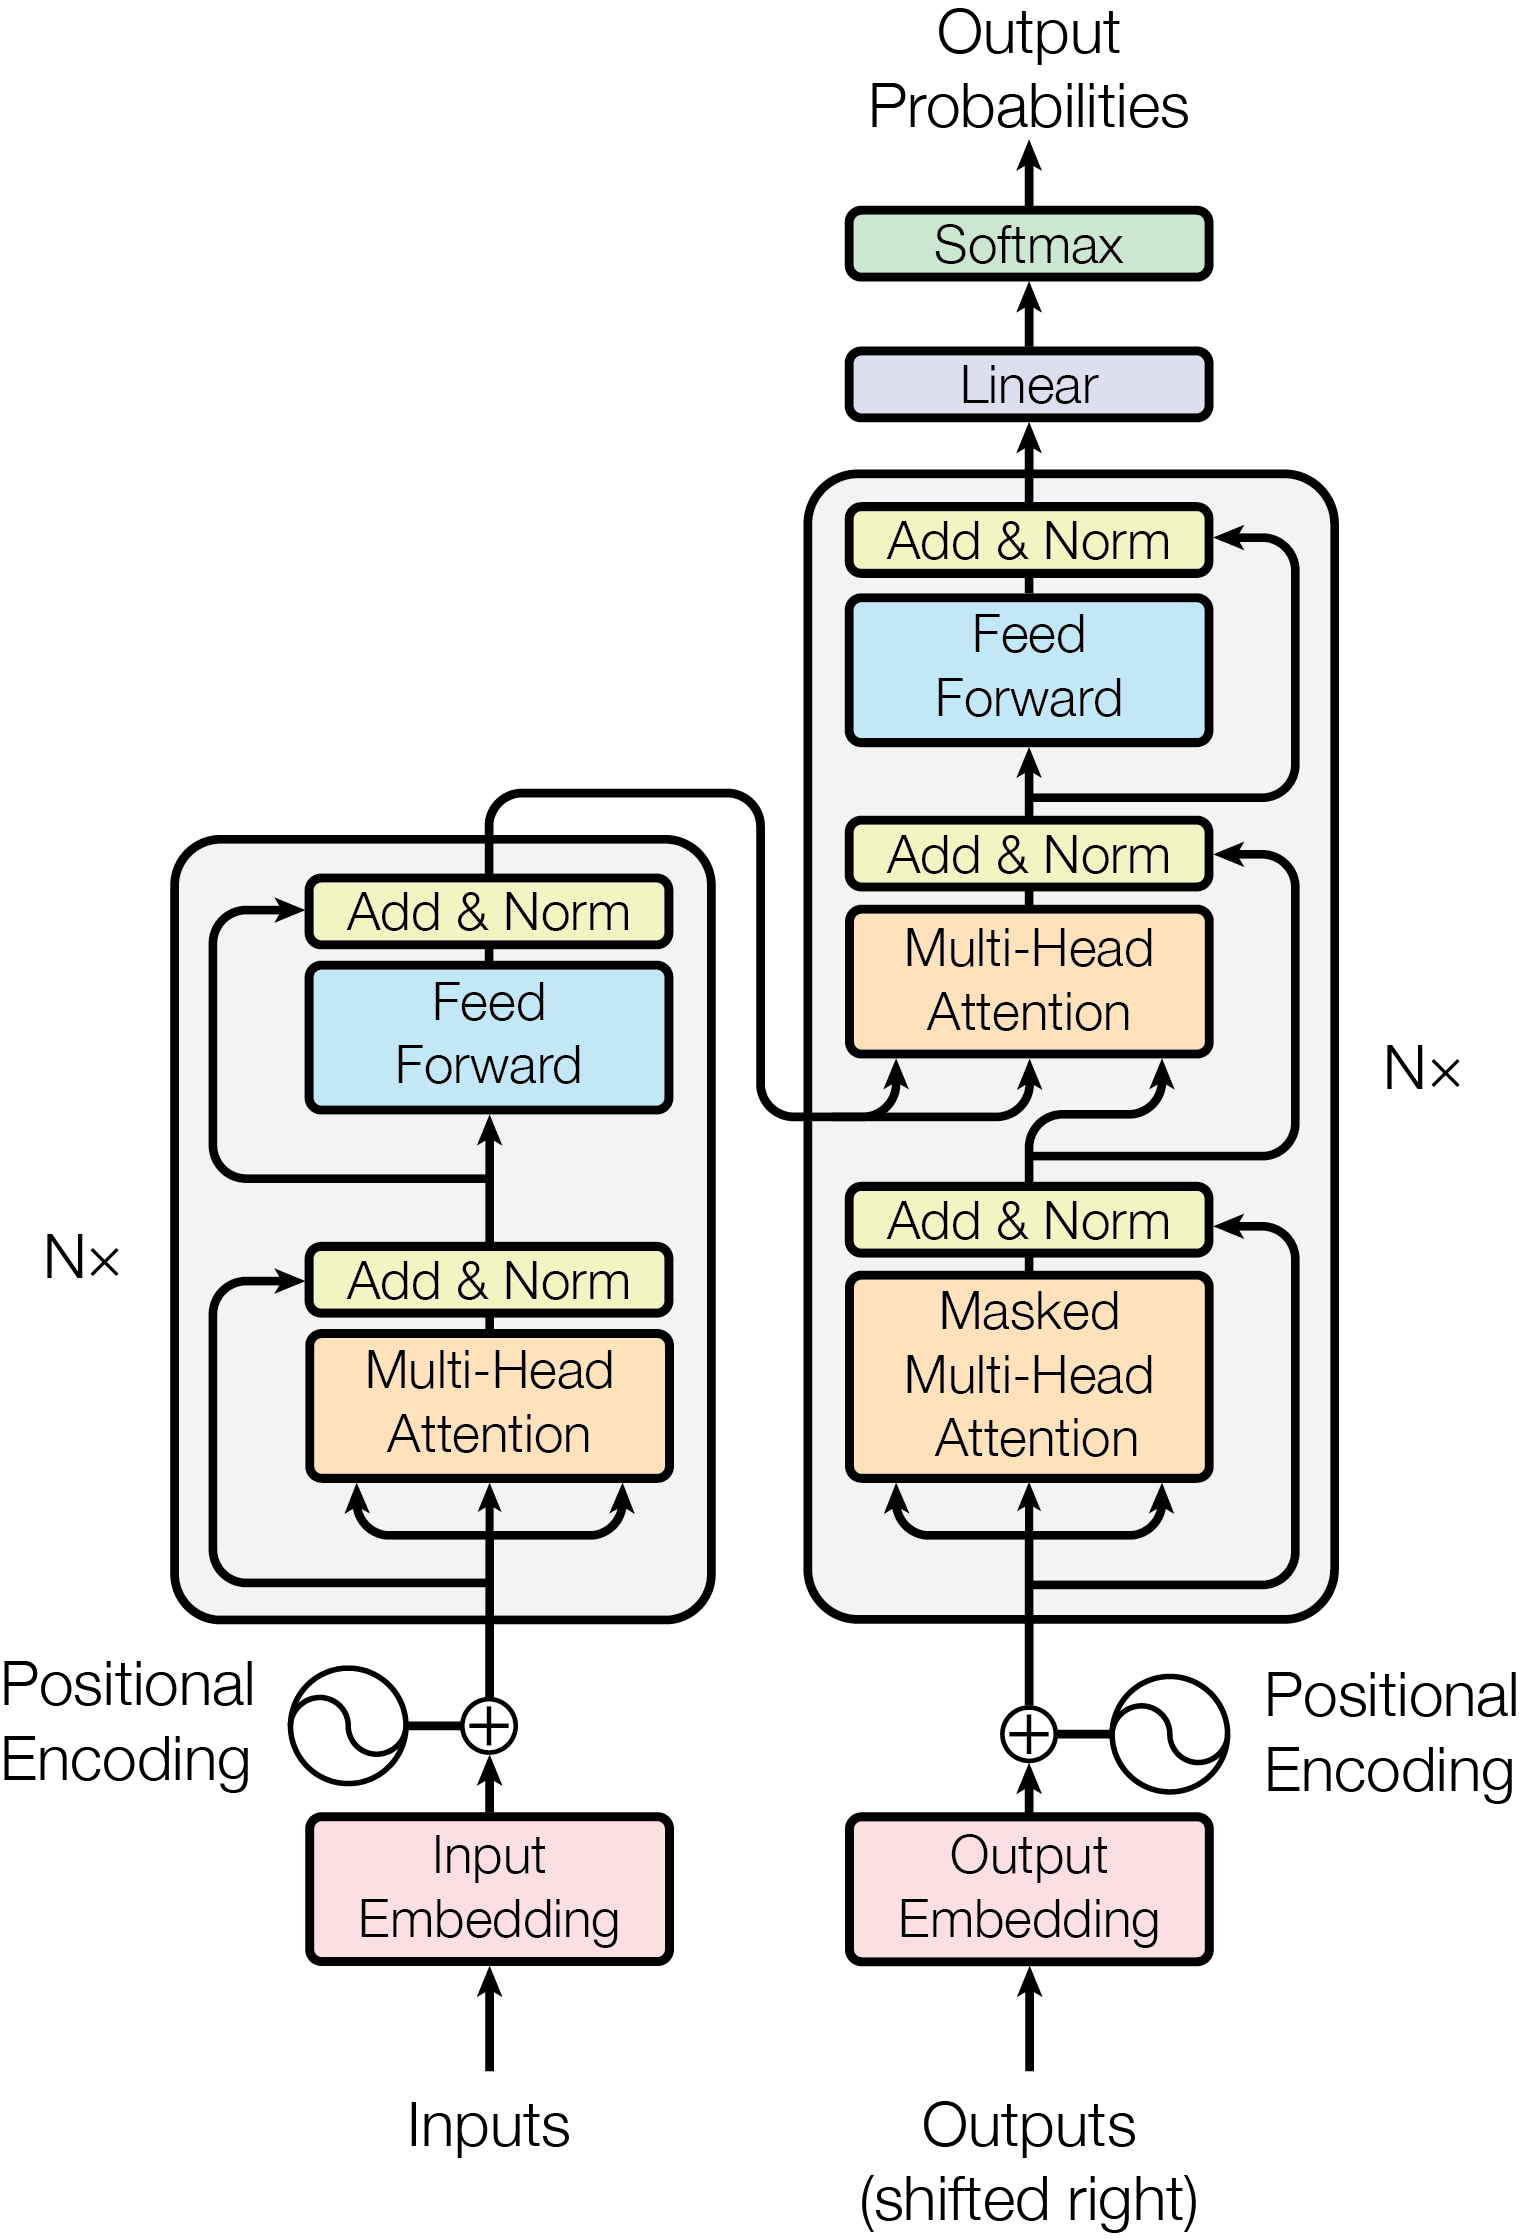
\includegraphics[width=0.4\linewidth]{./img/transformer.png}
        \end{figure}

    \item[Autoregressive generation] \marginnote{Autoregressive generation}
        A transformer generates the output sequence progressively given the input sequence and the past outputted tokens. At the beginning, the first token provided as the past output is a special start-of-sequence token. Generation is terminated when a special end-of-sequence token is generated.

        \begin{figure}[H]
            \centering
            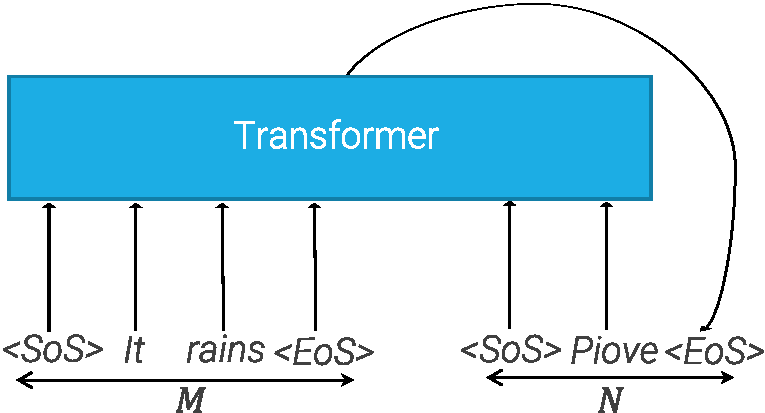
\includegraphics[width=0.3\linewidth]{./img/_transformer_autoregressive.pdf}
            \caption{Example of autoregressive generation}
        \end{figure}
\end{description}


\subsection{Attention mechanism}


\begin{description}
    \item[Traditional attention] \marginnote{Traditional attention}
        Matrix computed by a neural network to weigh each token of a sequence against the tokens of another one.

        \begin{figure}[H]
            \centering
            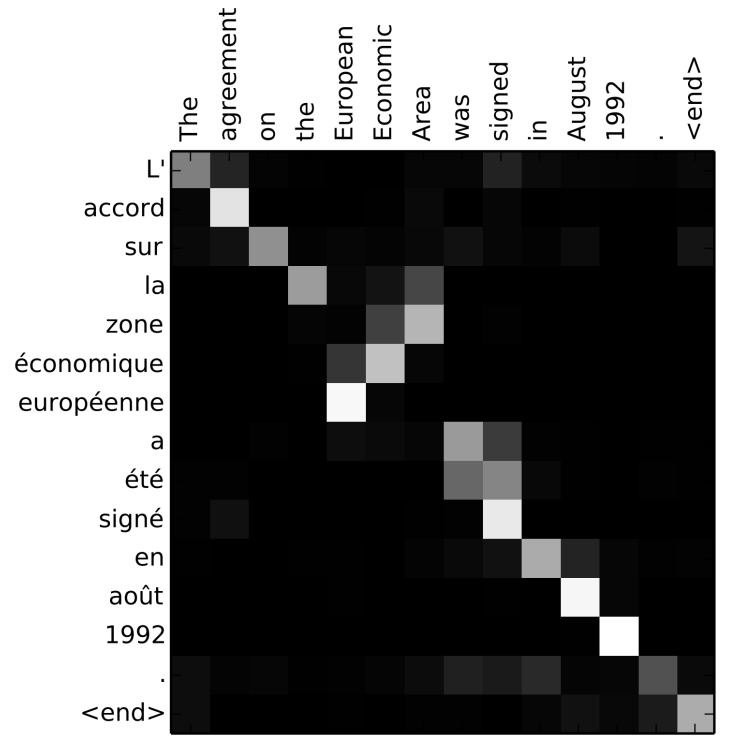
\includegraphics[width=0.3\linewidth]{./img/traditional_attention.png}
            \caption{Attention weights for machine translation}
        \end{figure}

        \begin{remark}
            Before attention, for tasks such as machine translation, the whole input sequence was mapped into an embedding that is used to influence the generation of the output.
        \end{remark}

        \begin{remark}
            This is not the same attention of transformers as they do not directly compute attention weights between inputs and outputs.
        \end{remark}

    \item[Dot-product attention] \marginnote{Dot-product attention}
        Given $M$ input tokens $\matr{Y} \in \mathbb{R}^{M \times d_Y}$ and a vector $\vec{x}_1 \in \mathbb{R}^{d_Y}$, dot-product attention computes a linear combination of $\matr{Y}$ where each component is weighted based on a similarity score between $\matr{Y}$ and $\vec{x}_1$.

        This is done as follows:
        \begin{enumerate}
            \item Determine the similarity scores of the inputs as the dot-product between $\vec{x}_1$ and $\matr{Y}^T$:
                \[ \vec{x}_1 \matr{Y}^T \in \mathbb{R}^{M} \]
            \item Compute the attention weights by applying the \texttt{softmax} function on the similarity scores:
                \[ \texttt{softmax}(\vec{x}_1 \matr{Y}^T) \in \mathbb{R}^{M} \]
            \item Determine the output activation $\vec{a}_1$ as the dot-product between the attention weights and the input $\matr{Y}$:
                \[ \mathbb{R}^{d_Y} \ni \vec{a}_1 = \texttt{softmax}(\vec{x}_1 \matr{Y}^T) \matr{Y} \]
        \end{enumerate}

        \begin{figure}[H]
            \centering
            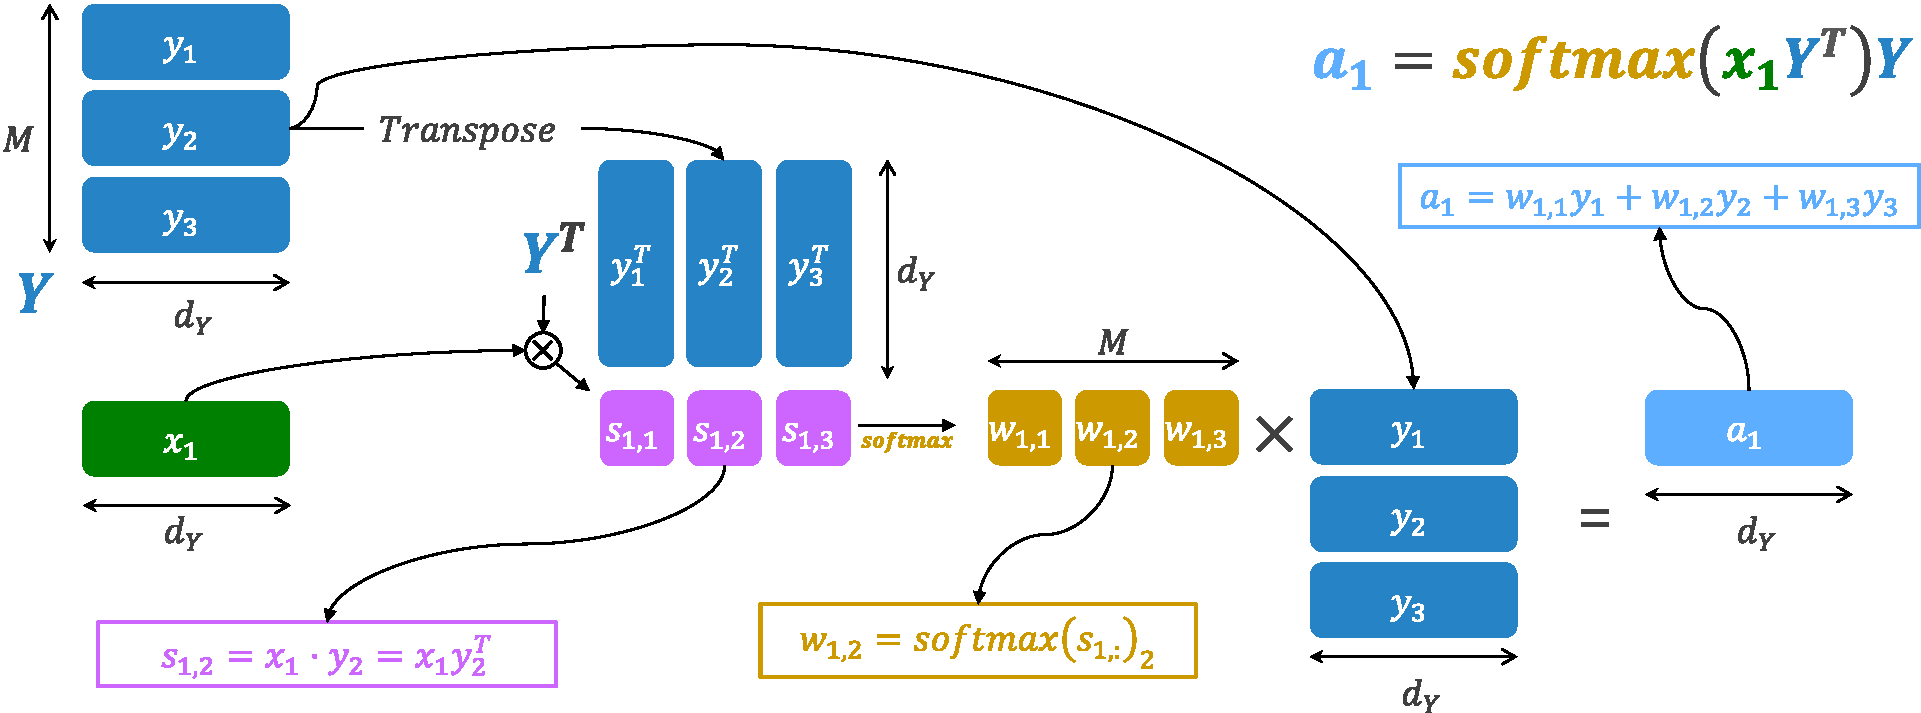
\includegraphics[width=0.8\linewidth]{./img/_dot_product_attention.pdf}
            % \caption{Steps of dot-product attention}
        \end{figure}

    \item[Scaled dot-product attention] \marginnote{Scaled dot-product attention}
        To add more flexibility, a linear transformation can be applied on the inputs $\matr{Y}$ and $\vec{x_1}$ to obtain:
        \begin{descriptionlist}
            \item[Keys] 
                With the projection $\matr{W}_K \in \mathbb{R}^{d_Y \times d_K}$ such that $\mathbb{R}^{M \times d_K} \ni \matr{K} = \matr{Y} \matr{W}_K$, where $d_K$ is the dimension of the keys.

            \item[Query] 
                With the projection $\matr{W}_Q \in \mathbb{R}^{d_X \times d_K}$ such that $\mathbb{R}^{d_K} \ni \vec{q}_1 = \matr{Y} \matr{W}_X$, where $d_X$ is the length of $\vec{x}_1$ that is no longer required to be $d_Y$ as there is a projection.

            \item[Values]
                With the projection $\matr{W}_V \in \mathbb{R}^{d_Y \times d_V}$ such that $\mathbb{R}^{M \times d_V} \ni \matr{V} = \matr{Y} \matr{W}_K$, where $d_V$ is the dimension of the values.
        \end{descriptionlist}

        The attention mechanism is then defined as:
        \[ \vec{a}_1 = \texttt{softmax}(\vec{q}_1 \matr{K}^T)\matr{V} \]

        To obtain smoother attention weights when working with high-dimensional activations (i.e., avoid a one-hot vector from \texttt{softmax}), a temperature of $\sqrt{d_K}$ is applied to the similarity scores:
        \[ \vec{a}_1 = \texttt{softmax}\left( \frac{\vec{q}_1 \matr{K}^T}{\sqrt{d_K}} \right)\matr{V} \]

        \begin{figure}[H]
            \centering
            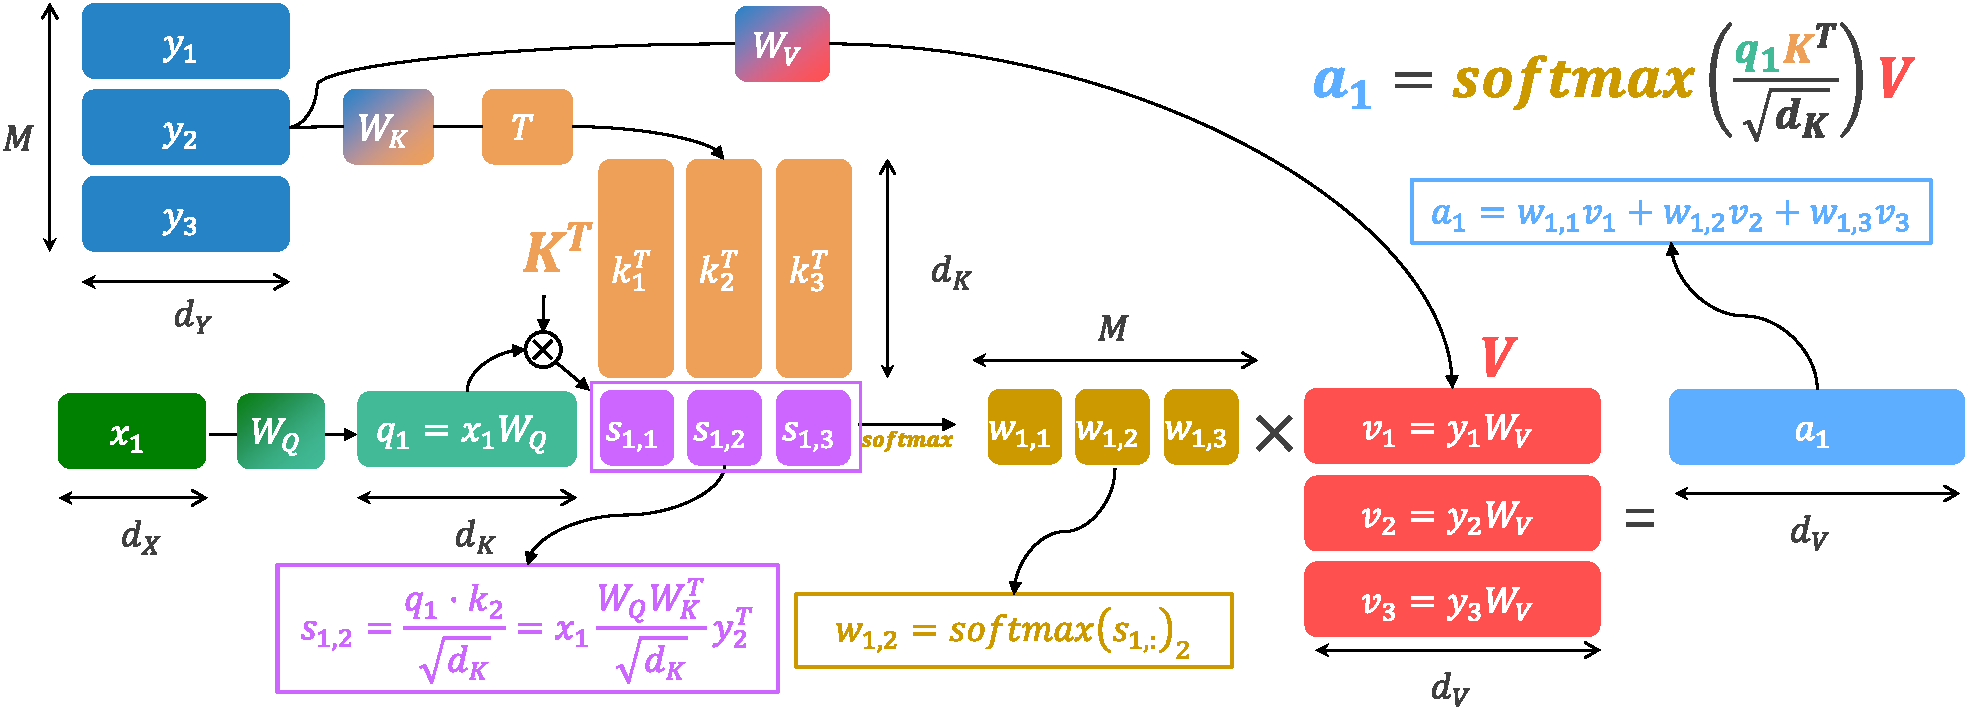
\includegraphics[width=0.8\linewidth]{./img/_scaled_dot_attention.pdf}
            % \caption{Steps of scaled dot-product attention}
        \end{figure}

        Finally, due to the linear projections, instead of a single vector there can be an arbitrary number $N$ of inputs $\matr{X} \in \mathbb{R}^{N \times d_X}$ to compute the queries $\mathbb{R}^{N \times d_K} \ni \matr{Q} = \matr{X} \matr{W}_Q$. This change affects the similarity scores $\matr{Q}\matr{K}^T \in \mathbb{R}^{N \times M}$ and the output activations $\matr{A} \in \mathbb{R}^{N \times d_V}$. 

        The overall attention mechanism can be defined as:
        \[ \matr{A} = \texttt{softmax}_\texttt{row-wise}\left( \frac{\matr{Q}\matr{K}^T}{\sqrt{d_K}} \right) \matr{V} \]

        \begin{figure}[H]
            \centering
            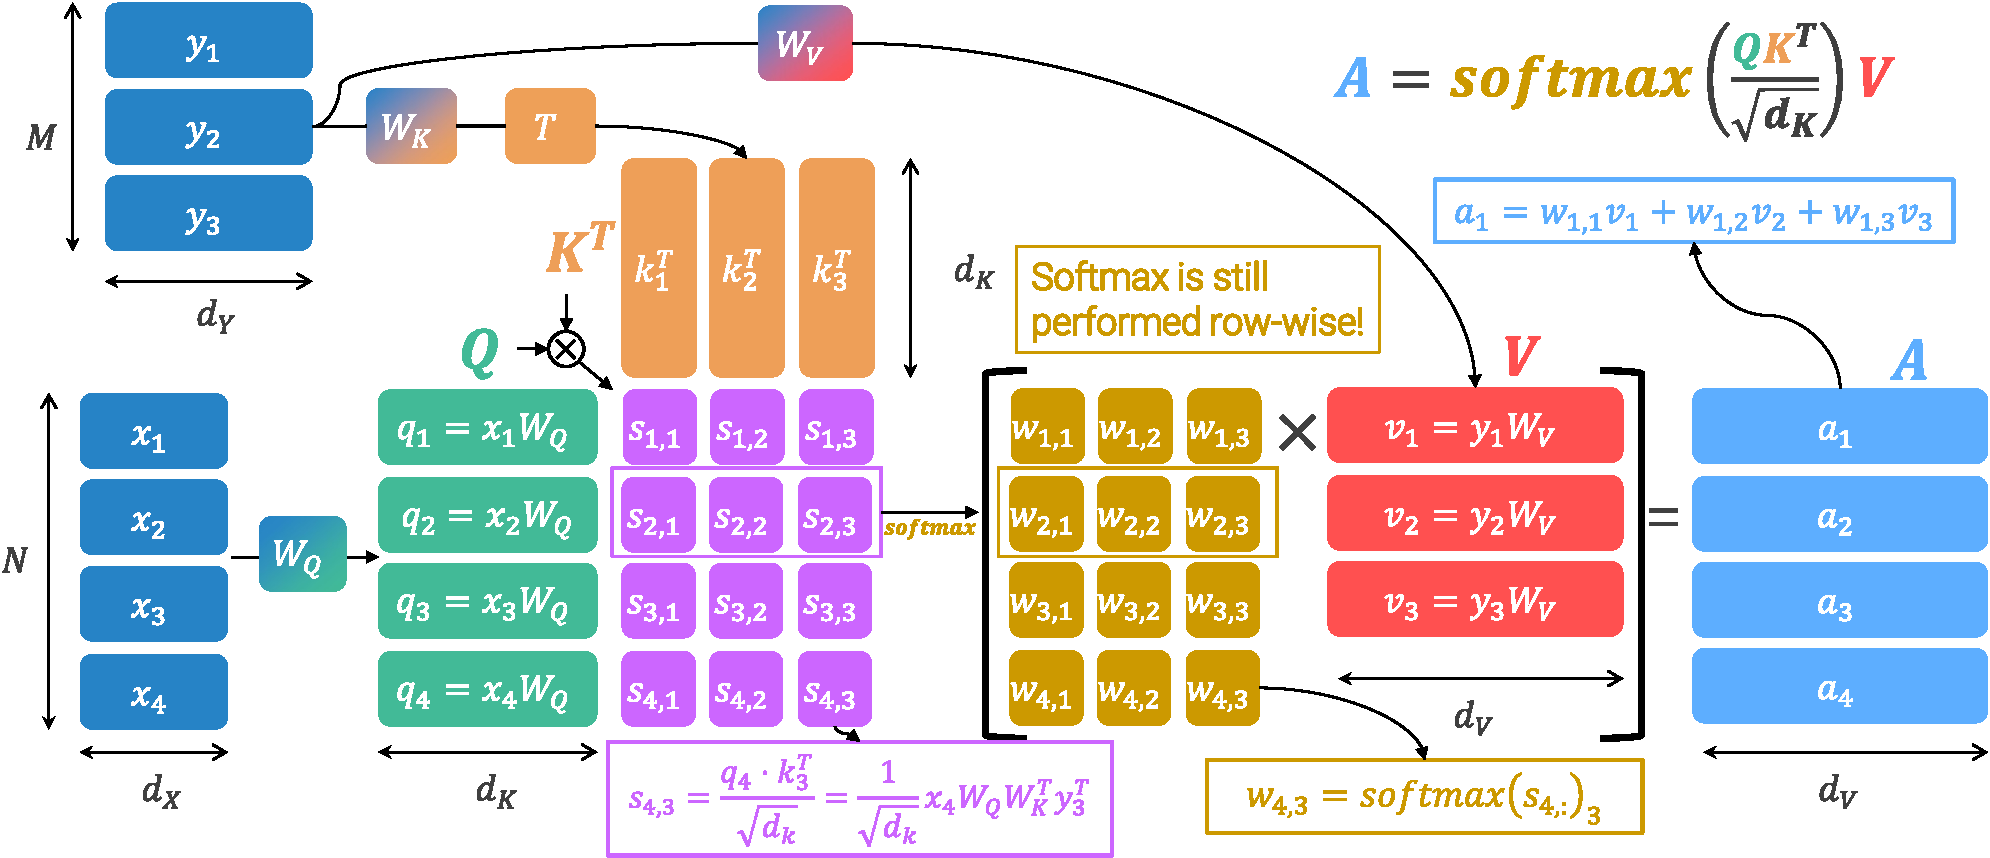
\includegraphics[width=0.8\linewidth]{./img/_scaled_dot_attention_multi_q.pdf}
            % \caption{Steps of scaled dot-product attention with multidimensional queries}
        \end{figure}

    \item[Self-attention] \marginnote{Self-attention}
        Scaled dot-product attention mechanism where the inputs to compute keys, queries, and values are the same.

        Given an input $\matr{Y} \in \mathbb{R}^{N \times d_Y}$, the shape of each component is: $\matr{K} \in \mathbb{R}^{N \times d_K}$, $\matr{Q} \in \mathbb{R}^{N \times d_K}$, $\matr{V} \in \mathbb{R}^{N \times d_V}$, and $\matr{A} \in \mathbb{R}^{N \times d_V}$.

        \begin{figure}[H]
            \centering
            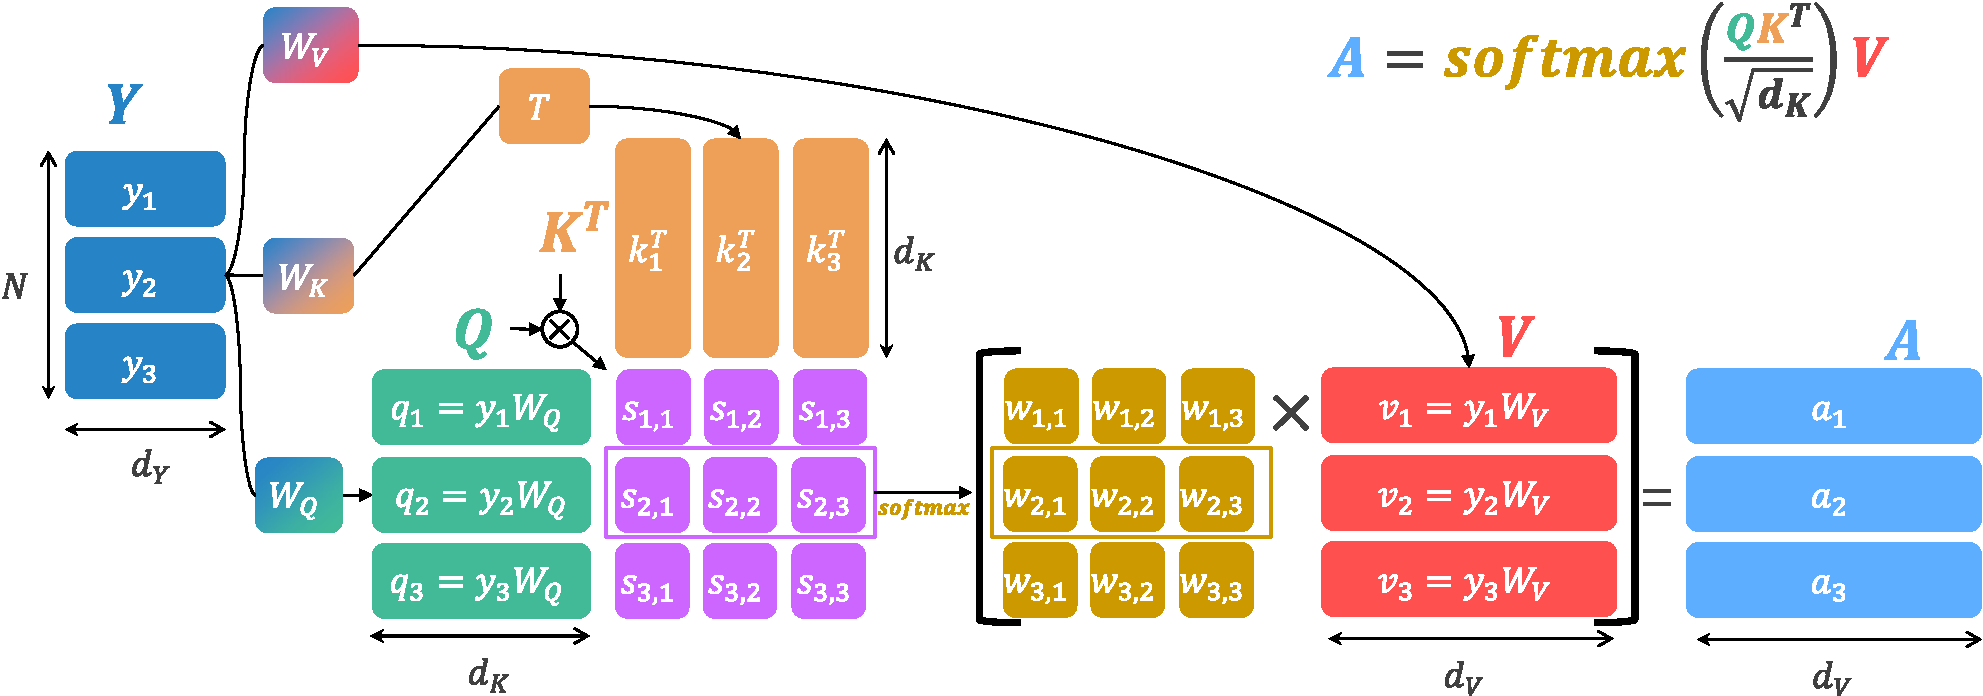
\includegraphics[width=0.8\linewidth]{./img/_self_attention.pdf}
            % \caption{Steps of self-attention}
        \end{figure}
\end{description}


\subsection{Embeddings}

\begin{description}
    \item[Embedding layer] \marginnote{Embedding layer}
        Converts input tokens into their corresponding learned embeddings of shape $d_Y$ (usually denoted as $d_\text{model}$).

        \begin{figure}[H]
            \centering
            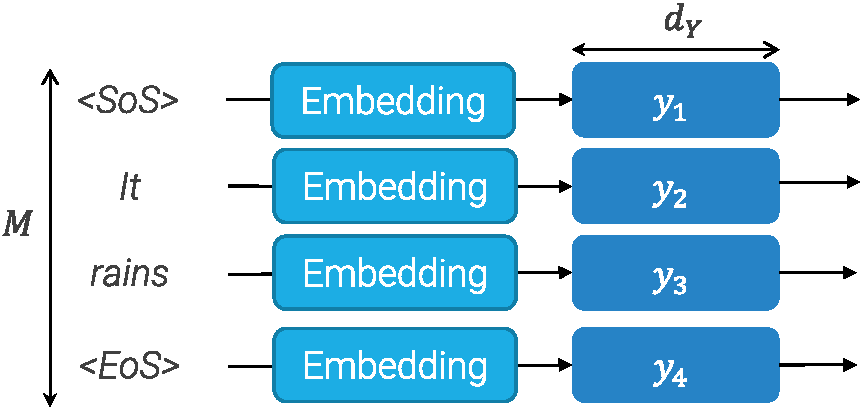
\includegraphics[width=0.4\linewidth]{./img/_transformer_embeddings.pdf}
        \end{figure}
\end{description}


\subsection{Encoder}

\begin{description}
    \item[Encoder components]
        A transformer encoder is composed of:

        \begin{description}
            \item[Multi-head self-attention (\texttt{MHSA})] \marginnote{Multi-head self-attention}
                Given an input $\matr{Y} \in \mathbb{R}^{M \times d_Y}$, a \texttt{MHSA} block parallelly passes it through $h$ different self-attention blocks to obtain the activations $\matr{A}^{(1)}, \dots, \matr{A}^{(h)}$. The output $\matr{A}$ of the block is obtained as a linear projection of the column-wise concatenation of the activations $\matr{A}^{(i)}$:
                \[ \mathbb{R}^{M \times d_Y} \ni \matr{A} = \left[ A^{(1)} \vert \dots \vert A^{(h)} \right] \matr{W}_O \]
                where $\matr{W}_O \in \mathbb{R}^{hd_V \times d_Y}$ is the projection matrix.

                \begin{figure}[H]
                    \centering
                    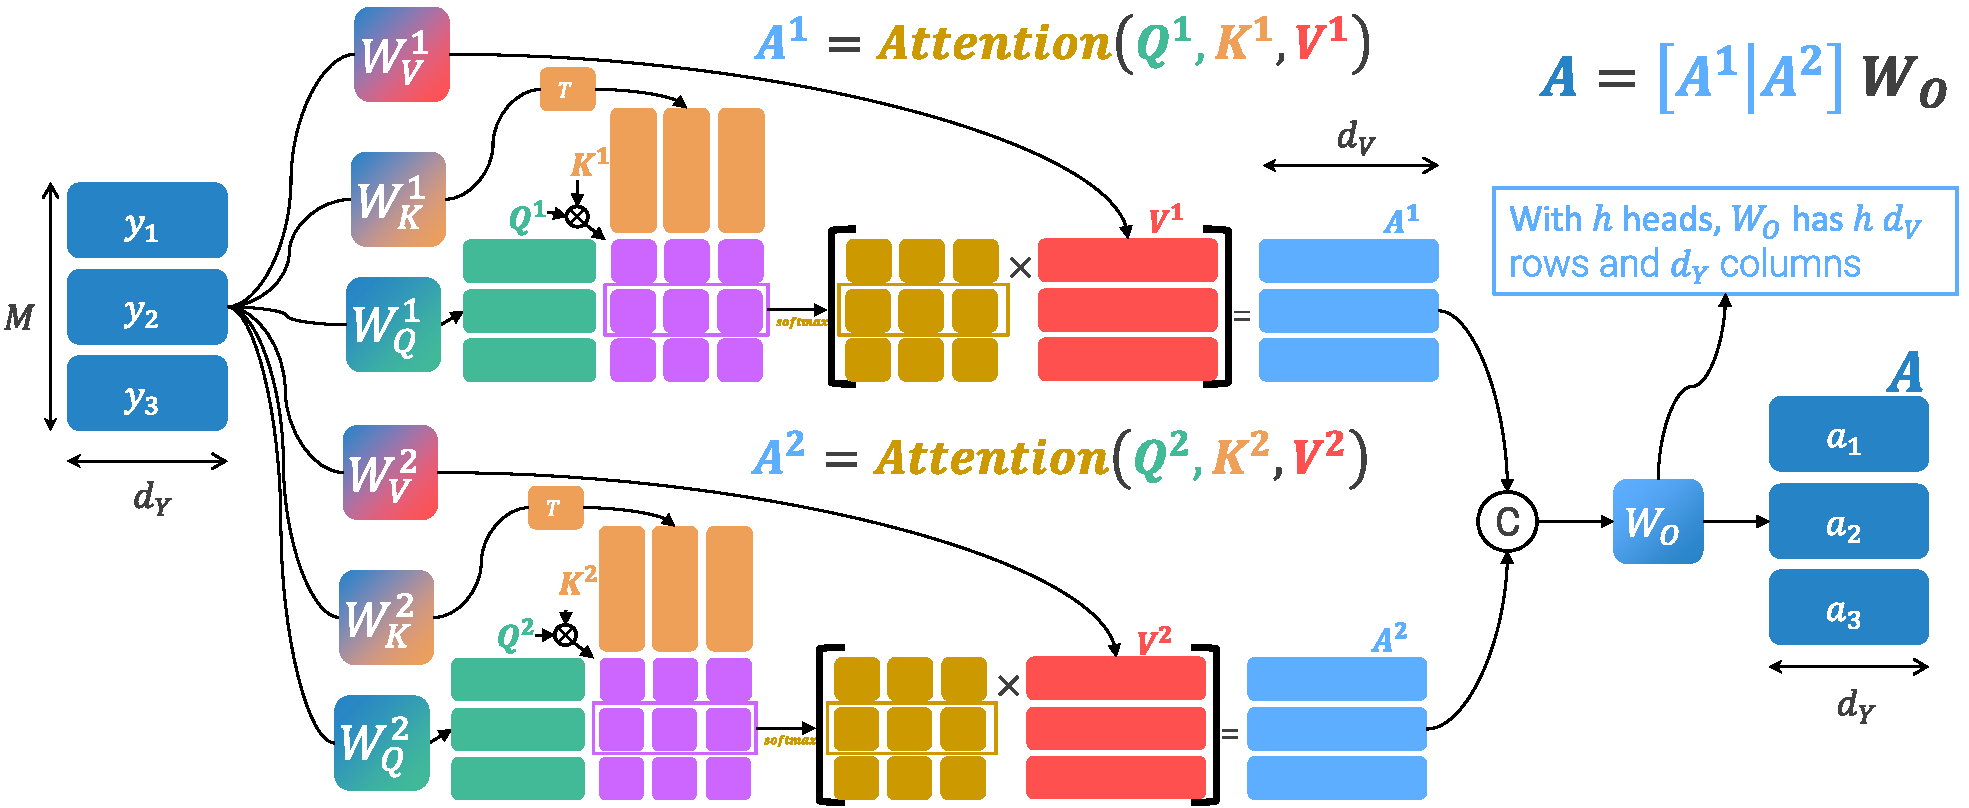
\includegraphics[width=0.7\linewidth]{./img/_multi_head_attention.pdf}
                    \caption{\texttt{MHSA} with two heads}
                \end{figure}

                \begin{remark}
                    The idea of multiple attention heads is to allow the model to attend to information from different representation subspaces.
                \end{remark}

                \begin{remark}
                    Even though they can be freely set, the dimensions for queries, keys, and values of each attention head usually are $d_K = d_V = d_Y/h$.
                \end{remark}

            \item[Layer normalization (\texttt{LN})] \marginnote{Layer normalization}
                Normalize each input activation independently to have zero mean and unit variance, regardless of the other activations in the batch.

                Given $B$ activations $\vec{a}^{(i)} \in \mathbb{R}^{D}$, mean and variance of each activation $i=1, \dots, B$ are computed as:
                \[ \mu^{(i)} = \frac{1}{D} \sum_{j=1}^{D} \vec{a}^{(i)}_{j} \qquad v^{(i)} = \frac{1}{D} \sum_{j=1}^{D} \left( \vec{a}^{(i)}_j - \mu^{(i)} \right)^2 \]
                Each component $j$ of the normalized activation $\hat{\vec{a}}^{(i)}$ is computed as:
                \[ \hat{\vec{a}}^{(i)}_{j} = \frac{\vec{a}^{(i)}_j - \mu^{(i)}}{\sqrt{v^{(i)} + \varepsilon}} \]
                As in batch normalization, the actual output activation $\vec{s}^{(i)}$ of each input $\vec{a}^{(i)}$ is scaled and offset by learned values:
                \[ \vec{s}^{(i)}_j = \vec{\gamma}_j \hat{\vec{a}}^{(i)}_j + \vec{\beta}_j \]

                \begin{remark}
                    Differently from computer vision, in NLP the input is not always of the same length and padding is needed. Therefore, batch normalization do not always work well.
                \end{remark}

                \begin{remark}
                    Layer normalization is easier to distribute on multiple computation units and has the same behavior at both train and inference time.
                \end{remark}

                \begin{figure}[H]
                    \centering
                    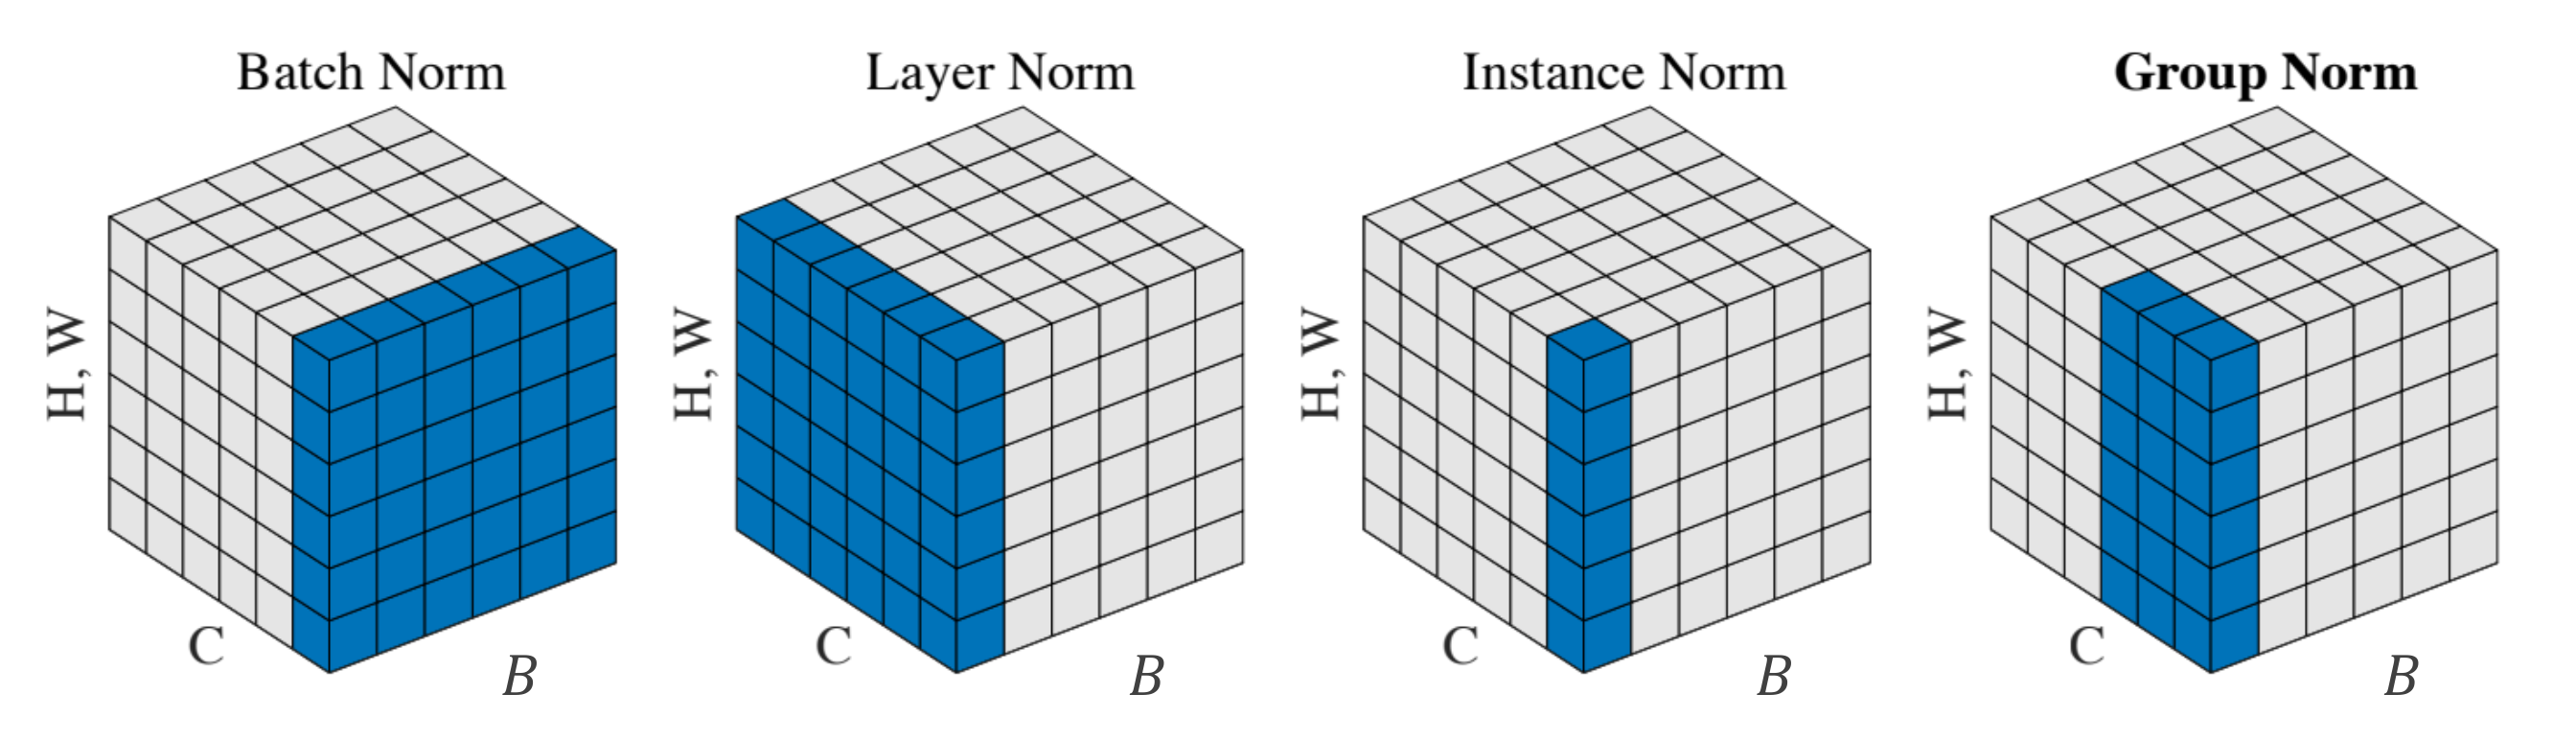
\includegraphics[width=0.8\linewidth]{./img/norm_methods.png}
                    \caption{Affected axis of normalization methods}
                \end{figure}

            \item[Feed-forward network (\texttt{FFN})] \marginnote{Feed-forward network}
                MLP with one hidden layer applied to each token independently. ReLU or one of its variants are used as activation function:
                \[ \texttt{FFN}(\vec{x}) = \texttt{relu}(\vec{x}\matr{W}_1 + \vec{b}_1)\matr{W}_2 + \vec{b}_2 \]

                \begin{remark}
                    It can be implemented using two 1D convolutions with kernel size $1$.
                \end{remark}

            \item[Residual connection] \marginnote{Residual connection}
                Around the \texttt{MHSA} and \texttt{FFN} modules.
        \end{description}


    \item[Encoder stack] \marginnote{Encoder stack}
        Composed of $L$ encoder layers.

    \item[Encoder layer] \marginnote{Encoder layer}
        Layer to compute a higher level representation of each input token while maintaining the same length of $d_Y$. 
        
        Given the input tokens $\matr{H}^{(i)} = [ \vec{h}^{(i)}_1, \dots, \vec{h}^{(i)}_N ]$, depending on the position of layer normalization, an encoder layer computes the following:
        \begin{descriptionlist}
            \item[Post-norm transformer] Normalization is done after the residual connection:
                \[
                    \begin{split}
                        \bar{\vec{h}}^{(i)}_j &= \texttt{LN}\left( \vec{h}^{(i)}_j + \texttt{MHSA}_{\matr{H}^{(i)}}(\vec{h}^{(i)}_j) \right) \\
                        \vec{h}^{(i+1)}_j &= \texttt{LN}\left( \bar{\vec{h}}^{(i)}_j + \texttt{FNN}(\bar{\vec{h}}^{(i)}_j) \right) \\
                    \end{split}
                \]

            \item[Pre-norm transformer] Normalization is done inside the residual connection:
                \[
                    \begin{split}
                        \bar{\vec{h}}^{(i)}_j &= \vec{h}^{(i)}_j + \texttt{MHSA}_{\matr{H}^{(i)}}\left( \texttt{LN}(\vec{h}^{(i)}_j) \right) \\
                        \vec{h}^{(i+1)}_j &= \bar{\vec{h}}^{(i)}_j + \texttt{FNN}\left( \texttt{LN}(\bar{\vec{h}}^{(i)}_j) \right) \\
                    \end{split}
                \]

                \begin{remark}
                    In practice, with pre-norm transformer training is more stable.
                \end{remark}
        \end{descriptionlist}

        \begin{figure}[H]
            \centering
            \begin{subfigure}{0.40\linewidth}
                \centering
                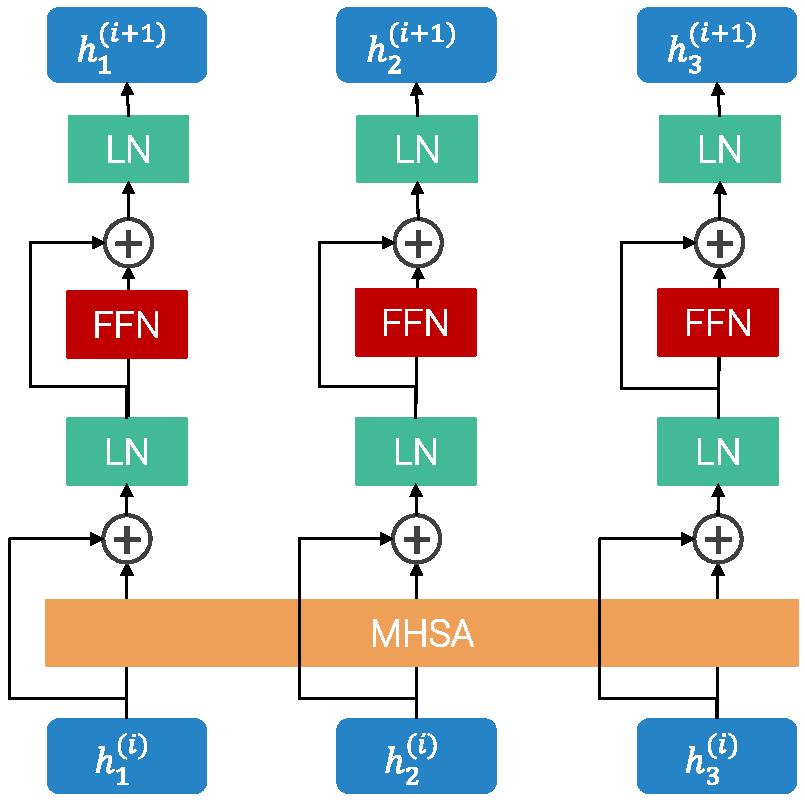
\includegraphics[width=0.8\linewidth]{./img/_post_norm_encoder.pdf}
                \caption{Encoder in post-norm transformer}
            \end{subfigure}
            \begin{subfigure}{0.40\linewidth}
                \centering
                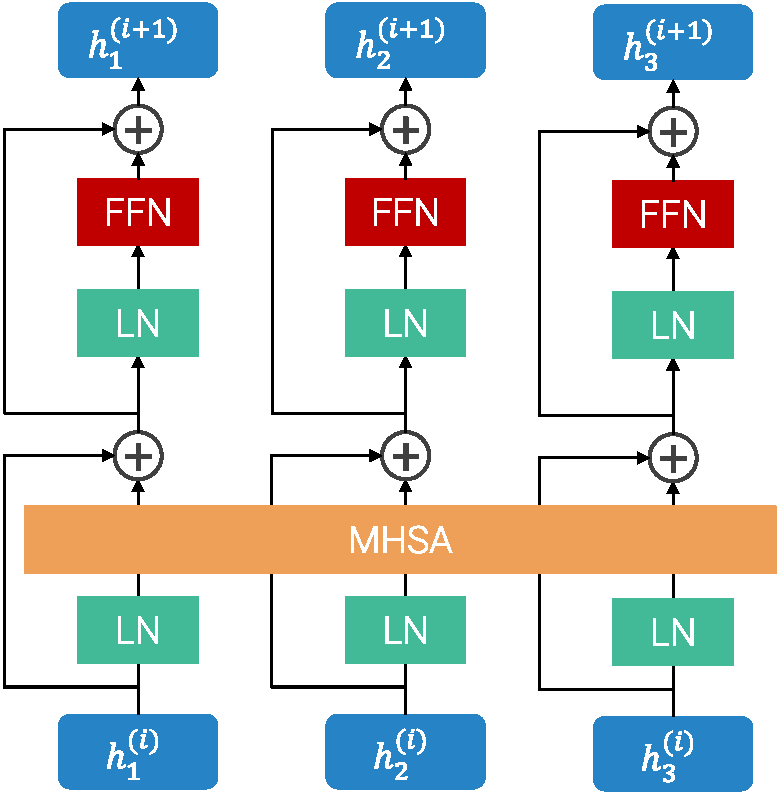
\includegraphics[width=0.8\linewidth]{./img/_pre_norm_encoder.pdf}
                \caption{Encoder in pre-norm transformer}
            \end{subfigure}
        \end{figure}


        \begin{remark}
            Of all the components in an encoder, attention heads are the only one that allow interaction between tokens.
        \end{remark}
\end{description}